%!TEX root = ../main.tex
%%%%%%%%%%%%%%%%%%%%%%%%%%%%%%%%%%
% Links: 
% https://www.geeksforgeeks.org/count-ways-reach-nth-stair/
% https://www.geeksforgeeks.org/count-ways-reach-nth-stair/
% https://www.geeksforgeeks.org/count-ways-reach-nth-stair-using-step-1-2-3/
% https://www.dailycodingproblem.com/blog/staircase-problem/
% https://leetcode.com/discuss/general-discussion/458695/Dynamic-Programming-Patterns
%
% Difficulty: Medium
% Companies: Amazon
%%%%%%%%%%%%%%%%%%%%%%%%%%%%%%%%%%

\chapter{Climb the Stairs}
\label{ch:stairs_climbing}
\section*{Introduction}
The problem covered by this chapter is a classical one, that has been asked during interview at big tech companies like Amazon or Google. It shares the underlying structure and key properties with many other problems and thus, not surprisingly, also its solution is very similar to theirs (for instance there is a one-to-one correnspondence with the coin change problem and the solution described in this chapter can be used to solve that problem too.). The tecniques discussed in the chapter can be applied to all problem which statements goes like this: \textit{Given a target find minimum (maximum) cost / path / sum to reach the target}. Usually the problem should be tackled by using the following approach: \textit{Choose minimum/maximum path among all possible paths before the current state, then add the value for the current state.}
Words like state and current will be clearer by the end of the chapter.

\section{Problem statement}
\label{sec:stairs_climbing_statement_easy}
\begin{exercise}
You are climbing a stair case and it takes $n$ steps to reach to the top.

Each time you can either climb $1$ or $2$ steps. In how many distinct ways can you climb to the top?


\begin{example}
	\hfill \\ 
	Given $n = 3$ the answer is $3$ because there are three ways (See Figure \ref{fig:stair_example_3} to climb to the top of the stairs:
	\begin{enumerate}
		\item $1$ step + $1$ step + $1$ step
		\item $1$ step + $2$ steps
		\item $2$ steps + $1$ step
	\end{enumerate}
	

	
\end{example}

\begin{example}
	\hfill \\
	Given $n = 4$ the answer is $5$ because there are five ways (See Figure \ref{fig:stair_example_5} to climb to the top of the stairs:
	\begin{enumerate}
		\item $1$ step + $1$ step + $1$ step + $1$ step
		\item $2$ steps + $1$ step + $1$ step
		\item $1$ step + $1$ step + $2$ steps 
		\item $1$ step + $2$ steps + $1$ step
		\item $2$ steps +  $2$ steps
	\end{enumerate}
	
	
\end{example}
\end{exercise}

\begin{figure}
	\centering
	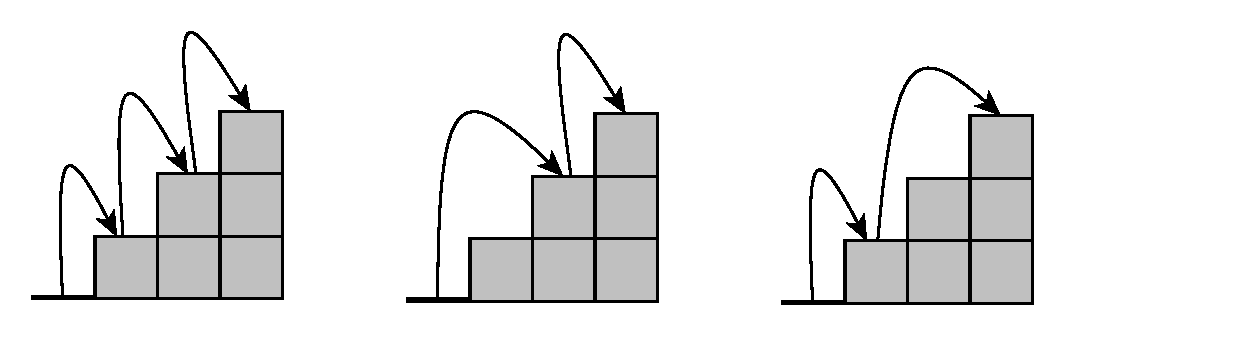
\includegraphics[width=\textwidth]{sources/stairs_climbing/images/stairs3}
	\caption{All different ways to climb a 3 stairs staricase using steps of size $1$ or $2$.}
	\label{fig:stair_example_3}
\end{figure}

\begin{figure}
	\centering
	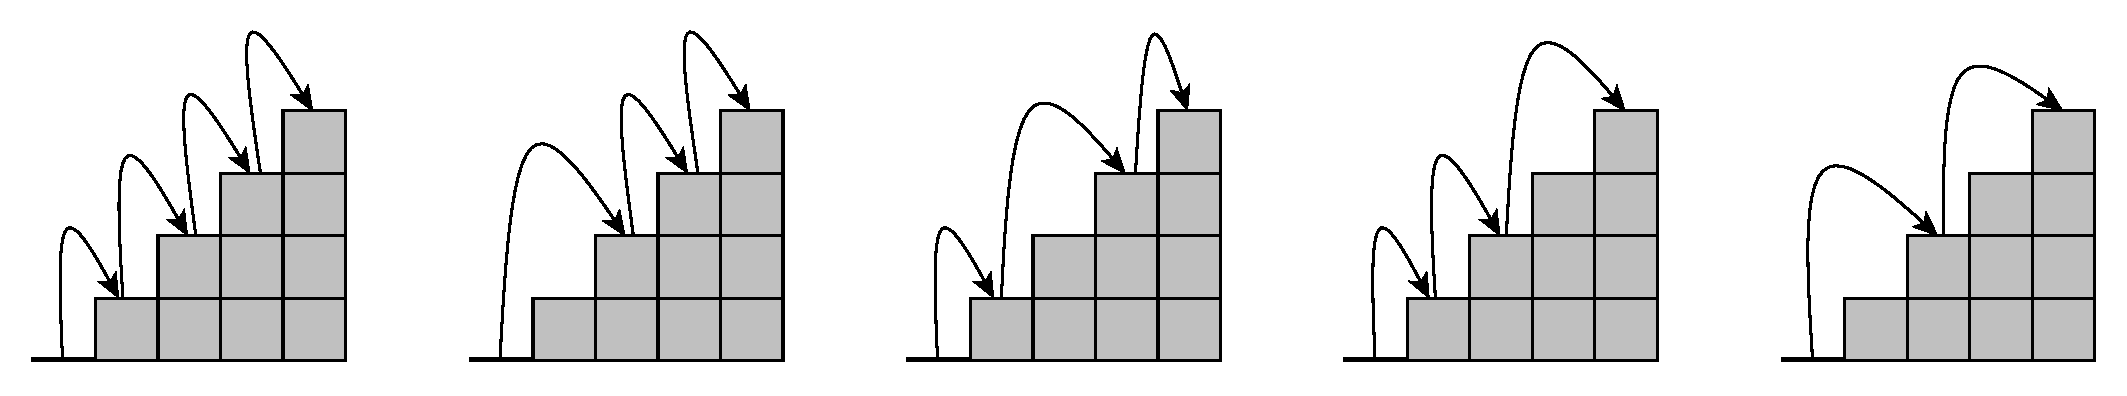
\includegraphics[width=\textwidth]{sources/stairs_climbing/images/stairs4}
	\caption{All different ways to climb a four stairs staricase using steps of size $1$ or $2$.}
	\label{fig:stair_example_5}
\end{figure}

\section{Clarification Questions}

\begin{QandA}
	\item \begin{questionitem} \begin{question} Can the size of the stair be zero?  \end{question} 	 
    \begin{answered}
		\textit{Yes, the staircase can be made of zero steps.}
	\end{answered} \end{questionitem}
	
	\item \begin{questionitem} \begin{question} It is guaranteed the answer to fit a built-in integer?  \end{question} 	 
    \begin{answered}
		\textit{Yes, do not worry about overflow.}
	\end{answered} \end{questionitem}

\end{QandA}

\section{Discussion}
\label{stairs_climbing:sec:discussion}

This is probably one problem that it is easier to tackle by first looking at a few examples so it is easier to see patterns. Table \ref{tab:stairs_climbing_ways_up_tp_7} shows  how many ways there are to climb a stair of lenght $n$ up to $n=7$.

\begin{table}
	\centering
	\begin{tabular}{|c|c|}
		\hline
		$n$ & \textbf{Ways} \\ \hline
		$0$ & $0$ \\ \hline
		$1$ & $1$ \\ \hline
		$2$ & $2$ \\ \hline
		$3$ & $3$ \\ \hline
		$4$ & $5$ \\ \hline
		$5$ & $8$ \\ \hline
		$6$ & $13$ \\ \hline
		$7$ & $21$ \\ \hline
	\end{tabular}
\label{tab:stairs_climbing_ways_up_tp_7}
\caption{All the ways to climb a stair of lenght $n \leq 7$ }
\end{table}

Looking at the table one thing should be immediately noticed i.e. the number of ways to climb the stair of size $n$ is equal to the $n^th$ element of the \textbf{Fibonacci} sequence (starting with two $1$).
Once tht is clear then the solution is straightforward as shown in Listing \ref{list:stairs_climbing_fibonacci}.

\lstinputlisting[language=c++, caption=Solution to the stairs climbining problem with steps of size $1$ and $2$ using Fibonacci.,label=list:stairs_climbing_fibonacci]{sources/stairs_climbing/stairs_climbing_solution1.cpp}

Now, let's have a look at why the seemingly unrelated fibonacci sequence plays a role in this problem. If the problem is looked at as an iterative process in which at each step a certain number of stairs are climbed. For instance if $n = 3$ and:
\begin{itemize}
	\item[-] $1$ step is hopped then the number of remaining steps is $3-1 = 2$. 
	\item[-] $2$ steps are hopped then the number of remaining steps is $3-2 = 1$.
\end{itemize}
When one step is hopped, the problem changes from climbing $n$ stairs to $n-1$ stairs. At this point the problem is seemingly unchanged except for the number of stairs left to climb and the same reasoning can be applied again:
\begin{itemize}
	\item[-] $1$ step is hopped then the number of remaining steps is $(n-1)-1 = n-2$. 
	\item[-] $2$ steps are hopped then the number of remaining steps is $(n-1)-2 = (n-3)$.
\end{itemize}
As can be seen, two decisions are possible i.e. climbing one or two stairs, exactly like in the fibinacci sequence, until either the $n$ step or a point past to it is reached.

\section{Common Variation
}
\subsection{Arbitrary step lengths}
\label{stairs_climbing:sec:arbitrary_steps}
But what happens when the step sizes allowed are not just $1$ or $2$ but an array of $k$ positive values $A=\{s_1 < s_2 < \ldots < s_k\}$. The problem statement for this harder variant of the problem is as follows:

\begin{exercise}
You are climbing a stair case and it takes $n$ steps to reach to the top.

Each time you can either climb $s_1$ or $s_2$ or $\ldots$ or $s_k$ steps where $0 < s_1 < s_2 < \ldots < s_k$. In how many distinct ways can you climb to the top?
\end{exercise}

Note how this problem is equivalent to the easier version described in Section \ref{sec:stairs_climbing_statement_easy} when the allowed step sizes are $s_i = 1$ and $s_2=2$.

